\documentclass{beamer}
% \usetheme{Berkeley}
% \usetheme{Boadilla}
\usetheme{Madrid}
% \usetheme{Montpellier}
% \usetheme{Warsaw}
% \usetheme{Copenhagen}
% \usetheme{Goettingen}
% \usetheme{Hannover}
% \usetheme{PaloAlto}
% \usetheme{AnnArbor}
% \usetheme{Bergen}

%\usepackage{beamerthemesplit}


\usepackage{amscd,amsxtra,amsthm}
%\usepackage[all]{xy}
%\usepackage{etex}
%\usepackage{pictex}
\usepackage{graphicx}
\usepackage{mathtools}
\usepackage{enumitem}

\theoremstyle{conjecture1}
%\newtheorem{conjecture}[theorem]{Conjecture}
\newtheorem{conjecture1}[theorem]{Conjecture 1}
\theoremstyle{conjecture2}
%\newtheorem{conjecture}[theorem]{Conjecture}
\newtheorem{conjecture2}[theorem]{Conjecture 2}

\def\G{\widetilde{G}}
\def\B{\widetilde{B}}
\def\T{\widetilde{T}}
\def\b{\widetilde{b_* }}
\def\M{\overline{M}}
\def\C{\mathbb{C}}
\def\Q{\mathbb{Q}}
\def\Z{\mathbb{Z}}
\def\F{\mathbb{F}}
\def\I{\mathbb{I}}
\def\Q{\mathbb{Q}}
\def\N{\mathbb{N}}
\def\R{\mathbb{R}}
\def\s{\mbox{\bf s}}
\def\pr{\mbox{\bf p}}
\def\i{\mbox{\bf i}}
\def\k{\mbox{\bf k}}
\def\h{\mbox{\bf h}}
\def\e{\epsilon}
\def\vp{\varpi }
\def\O{\mathcal{O}}
\def\v{\upsilon }
\def\p{\wp }
\def\z{\zeta _\upsilon}
\def\d{\cdot}
\def\c{\bullet}
\def\a{\ast}




\title{Byzantine Generals Problem}
\author[ Graham Swain \\ \quad \\ WCU]{Graham Swain}
\date{October 15, 2022 \\ Math 479}

\begin{document}

\frame{\titlepage}

%%%%%%%%%%%%%%%%%%%%%%%%%%%%%%%%%%%%%%%%%%%%%%%%%%%%%%%%%%%%%%%%%%%%%%%%%%%%%%%%%%%%%%%%%%%%%%%%
%%  Introduction
%%%%%%%%%%%%%%%%%%%%%%%%%%%%%%%%%%%%%%%%%%%%%%%%%%%%%%%%%%%%%%%%%%%%%%%%%%%%%%%%%%%%%%%%%%%%%%%%

\section{Introduction}

\begin{frame}
    \begin{enumerate}[label={$\bullet$}]
        \item Byzantine armies are sieging a city.
        \item<2-> Generals can only communicate by sending messengers.
    \end{enumerate}
    
\end{frame}

\begin{frame}
    \begin{enumerate}[label={\Alph*.}]
        \item All loyal generals decide upon the same plan of action.
        \item<2-> A small number of traitors cannot cause the loyal generals to adopt a bad plan.
    \end{enumerate}
\end{frame}

\begin{frame}
    \begin{itemize}[label={$\bullet$}]
        \item Condition A is met by having the generals use the same method of decision making.
        \item<2-> Condition B is met by having the generals use a robust decision making method.
    \end{itemize}
\end{frame}

\begin{frame}
    To help ensure that Condition A and Condition B are met, we need to meet two other conditions:
    \begin{enumerate}[label={\arabic{enumi}.}]
        \item<2-> Every loyal general must obtain the same information $v_1,...,v_n$.
        \item<3-> {
            If the $i^{th}$ general is loyal, then the value that they send must be used by every loyal 
            general as the value of $v_i$.
        }
    \end{enumerate}
    \vspace{10pt}
    \only<4-> {Condition 1 can be rewritten as:}
    \begin{enumerate}[label={\arabic{enumi}$^\prime$.}]
        \item<4-> For every $i$, any two loyal generals use the same value of $v_i$.
    \end{enumerate} 
\end{frame}

\begin{frame}
    \begin{itemize}[label={$\bullet$}]
        \item Loyal generals cannot take a value $v_i$ at face value.
        \item<2-> {
            Condition 1$^\prime$ and Condition 2 are both contingent on a single $v_i$ sent by the $i^{th}$
            general.
        } 
    \end{itemize}
\end{frame}

\begin{frame}
    \begin{block}{Byzantine Generals Problem}
        \only<2-> {A commanding general must send an order to their $n - 1$ lieutenants such that:}

        \only<3-> {
            \begin{enumerate}[label={IC\arabic{enumi}.}]
                \item<3-> All loyal lieutenants obey the same order.
                \item<4-> If the commander is loyal, then every loyal lieutenant obeys the order they send.
            \end{enumerate}
        }
    \end{block}
\end{frame}

%%%%%%%%%%%%%%%%%%%%%%%%%%%%%%%%%%%%%%%%%%%%%%%%%%%%%%%%%%%%%%%%%%%%%%%%%%%%%%%%%%%%%%%%%%%%%%%%
%%  Three Generals
%%%%%%%%%%%%%%%%%%%%%%%%%%%%%%%%%%%%%%%%%%%%%%%%%%%%%%%%%%%%%%%%%%%%%%%%%%%%%%%%%%%%%%%%%%%%%%%%

\section{Three Generals}

\begin{frame}
    \vfill
    \centering
    \begin{beamercolorbox}[sep=8pt,center,shadow=true,rounded=true]{title}
        \usebeamerfont{title}Three Generals Problem\par%
    \end{beamercolorbox}

    \begin{figure}
        \centering
        \includegraphics[scale=.35]{../figures/three_generals.pdf}
    \end{figure}
\end{frame}


\begin{frame}
    \frametitle{Situation 1: Commander is Loyal}
    \begin{figure}
        \centering
        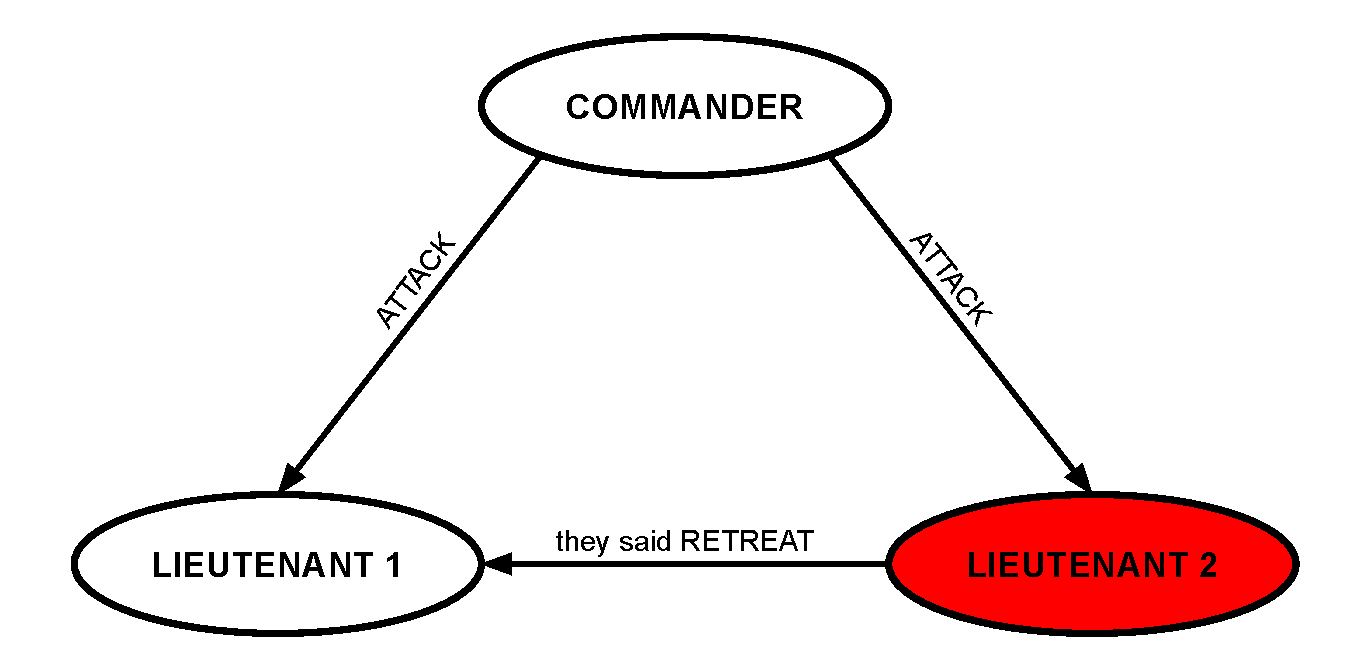
\includegraphics[scale=.5]{../figures/three_generals_loyal_commander.pdf}
    \end{figure}
\end{frame}

\begin{frame}
    \frametitle{Situation 1: Commander is a Traitor}
    \begin{figure}
        \centering
        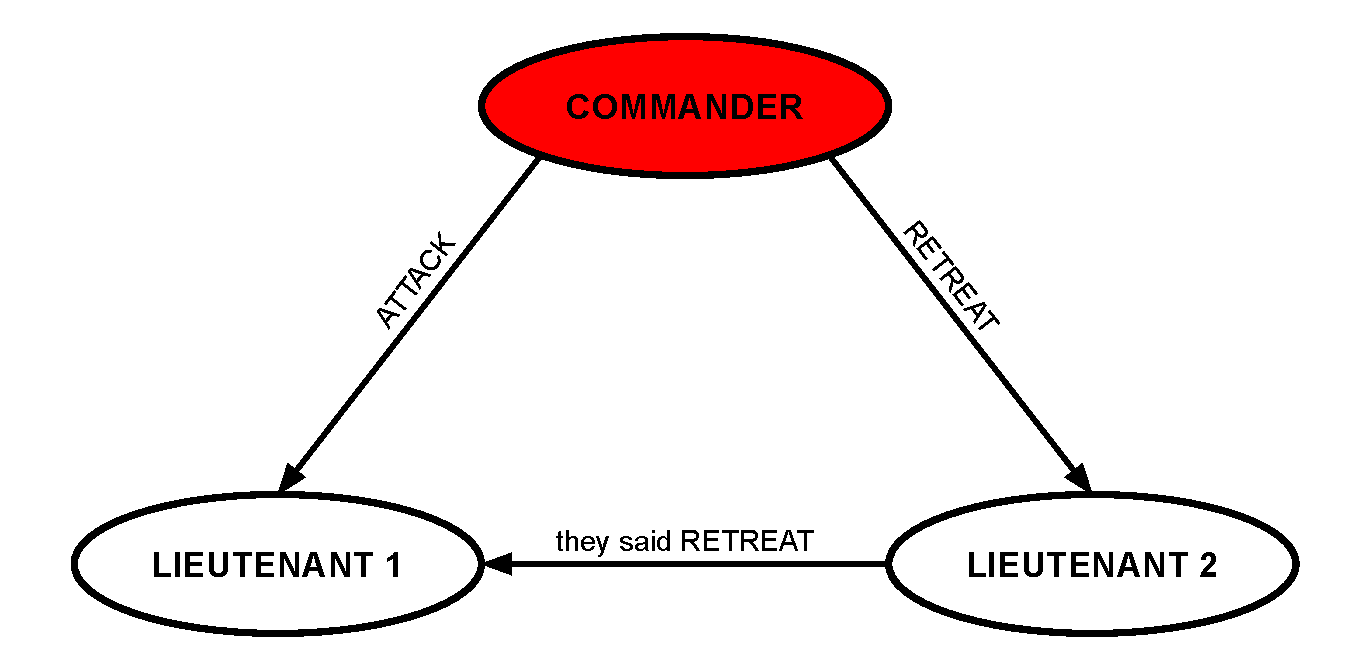
\includegraphics[scale=.5]{../figures/three_generals_unloyal_commander.pdf}
    \end{figure}
\end{frame}

\begin{frame}
    \begin{figure}
        \centering
        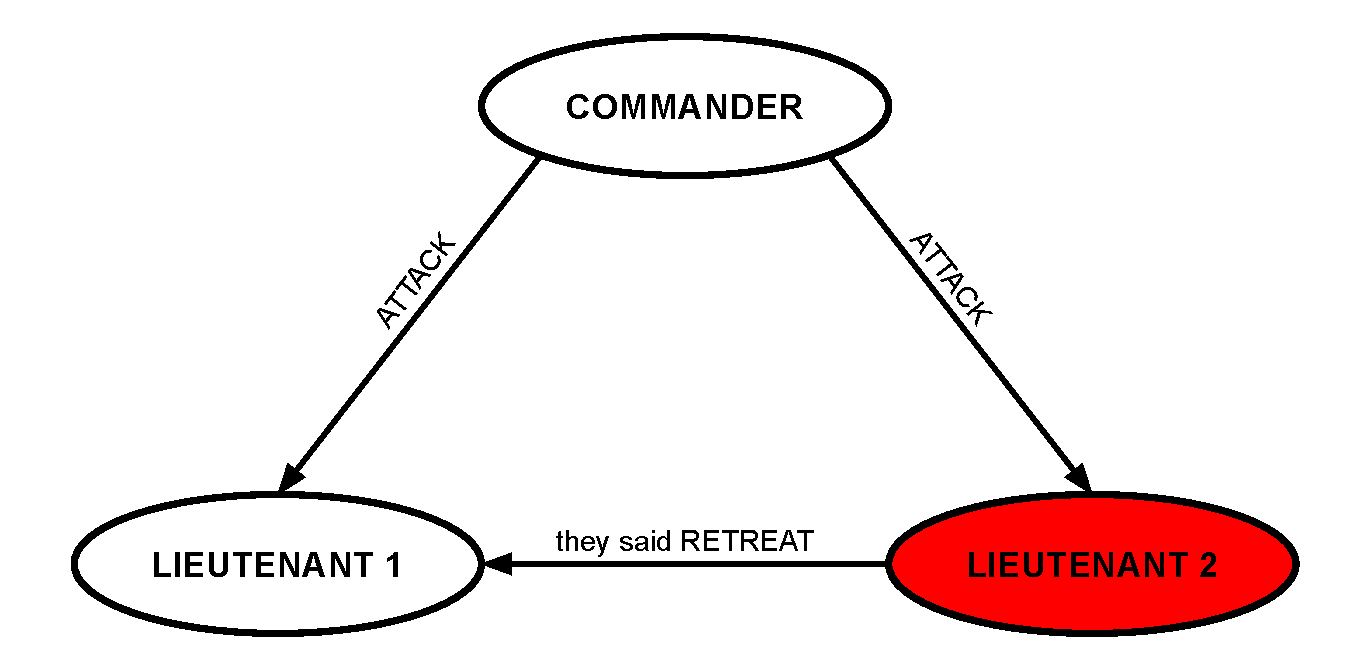
\includegraphics[scale=.35]{../figures/three_generals_loyal_commander.pdf}
    \end{figure}
    \begin{figure}
        \centering
        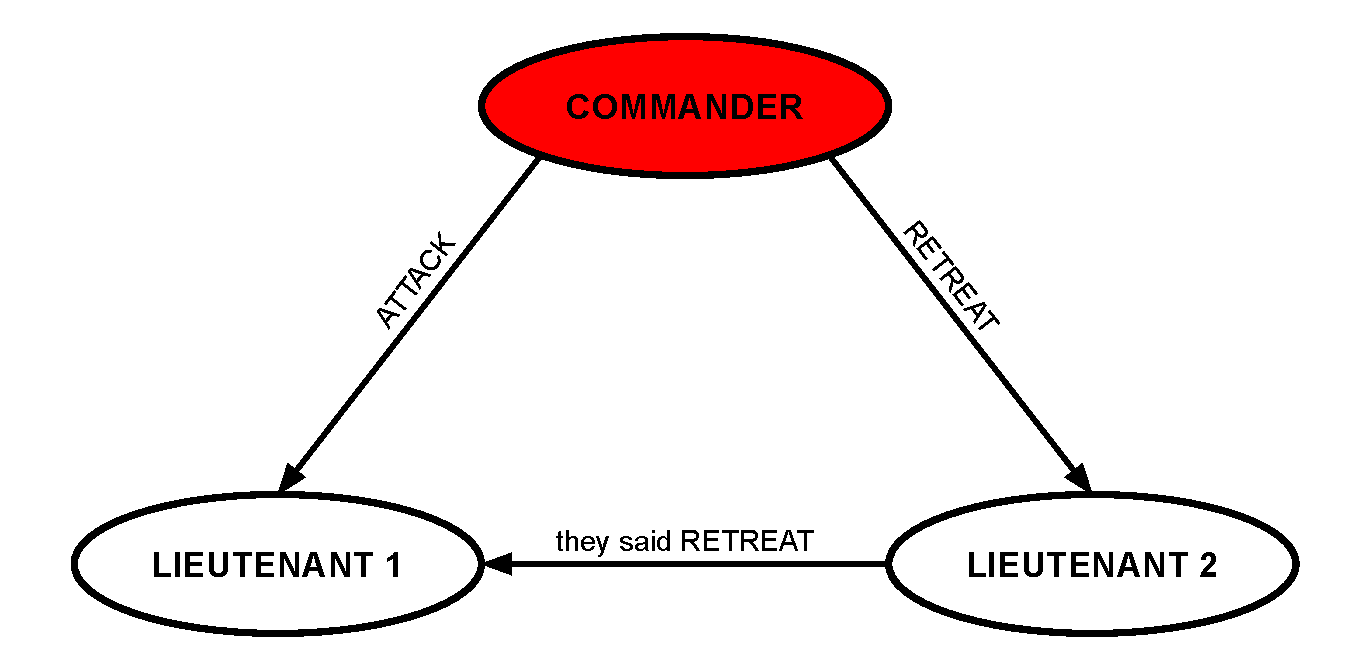
\includegraphics[scale=.35]{../figures/three_generals_unloyal_commander.pdf}
    \end{figure}
\end{frame}

\begin{frame}
    \begin{theorem}[Three Generals]
        No solution exists for $n<3m+1$ generals with $m$ traitors and $n>3$.
    \end{theorem}
\end{frame}

\begin{frame}
    \begin{proof}
        \only<1> {
            Assume that a solution exists for $3m$ or less Albanian generals. \\
            We will show a solution exists for three Byzantine generals with a single traitor. \\
        }
        

        \only<2-4> {
            Each Byzantine general represents at most $m$ Albanian generals. 
        }

        \only<3-4> {
            \vspace{12pt}
            Since the Albanian commander needs to be represented as well, the Byzantine commander represents 
            the Albanian commander as well as at most $m-1$ Albanian lieutenants. \\
        }

        \only<4> {
            \vspace{12pt}
            We know that there is a single Byzantine traitor. \\
            Since each Byzantine general represents at most $m$ Albanian generals, we know there is at 
            most $m$ Albanian traitors. \\
        }

        \only<5> {
            The assumed solution means that IC1 and IC2 is true for the Albanian generals. \\
            Since up to $m$ Albanian generals are represented by a Byzantine general, then IC1 and IC2 
            must also be true for the Byzantine generals, which we know is impossible, forming a contradiction.
        }
        \alt<5>{\qedhere}{\phantom\qedhere}
    \end{proof}
\end{frame}

\begin{frame}
    We know we need $n\geq3m+1$ generals if we have $m$ traitors.
\end{frame}


%%%%%%%%%%%%%%%%%%%%%%%%%%%%%%%%%%%%%%%%%%%%%%%%%%%%%%%%%%%%%%%%%%%%%%%%%%%%%%%%%%%%%%%%%%%%%%%%
%%  Oral Solution
%%%%%%%%%%%%%%%%%%%%%%%%%%%%%%%%%%%%%%%%%%%%%%%%%%%%%%%%%%%%%%%%%%%%%%%%%%%%%%%%%%%%%%%%%%%%%%%%

\section{Oral Solution}

\begin{frame}[t]
    \vfill
    \centering
    \begin{beamercolorbox}[sep=8pt,center,shadow=true,rounded=true]{title}
        \usebeamerfont{title}Oral Solution\par%
    \end{beamercolorbox}
\end{frame}

\begin{frame}
    We make some assumptions about the messages:
    \begin{enumerate}[label={A\arabic{enumi}.}]
        \item<2-> Every message that is sent is delivered correctly.
        \item<3-> The receiver of a message knows who sent it.
        \item<4> The absence of a message can be detected.
    \end{enumerate}
\end{frame}

\begin{frame}
    \begin{block}{Algorithm OM(0)}
        \begin{enumerate}[label=\arabic{enumi}.]
            \item<2-> The commander sends their value to every lieutenant.
            \item<3> {
                Each lieutenant uses the value they received from the commander. If they received no value, 
                default to RETREAT.
            }
        \end{enumerate}
    \end{block}
\end{frame}

\begin{frame}
    \begin{block}{Algorithm OM($m$), $m>0$}
        \begin{enumerate}[label=\arabic{enumi}.]
            \item<1-> The commander sends their value to every lieutenant.
            \item<2-> For each $i$,
            \begin{enumerate}[label={\alph*.}]
                \item<3-> {
                    Lieutenant $i$ receives a value $v_i$ from the commander. Default to RETREAT if they receive
                    no value.
                }
                \item<4-> {
                    Lieutenant $i$ acts as the commander in OM($m-1$) to send the message to each of the remaining
                    $n-2$ lieutenants.
                }
            \end{enumerate}
            \item<5-> For each $i$, and each $j$ not equal to $i$,
            \begin{enumerate}[label={\alph*.}]
                \item<6-> {
                    let $v_j$ be the value Lieutenant $i$ received from \\ Lieutenant $j$ in step (2b). Default to 
                    RETREAT if Lieutenant $i$ received no value from Lieutenant $j$.
                }
                \item<7-> Lieutenant $i$ uses the value $majority(v_1,...,v_{n-1})$.
            \end{enumerate}  
        \end{enumerate} 
    \end{block}
\end{frame}

\begin{frame}
    \frametitle{OM($m$) Commander is Loyal}
    \begin{figure}
        \centering
        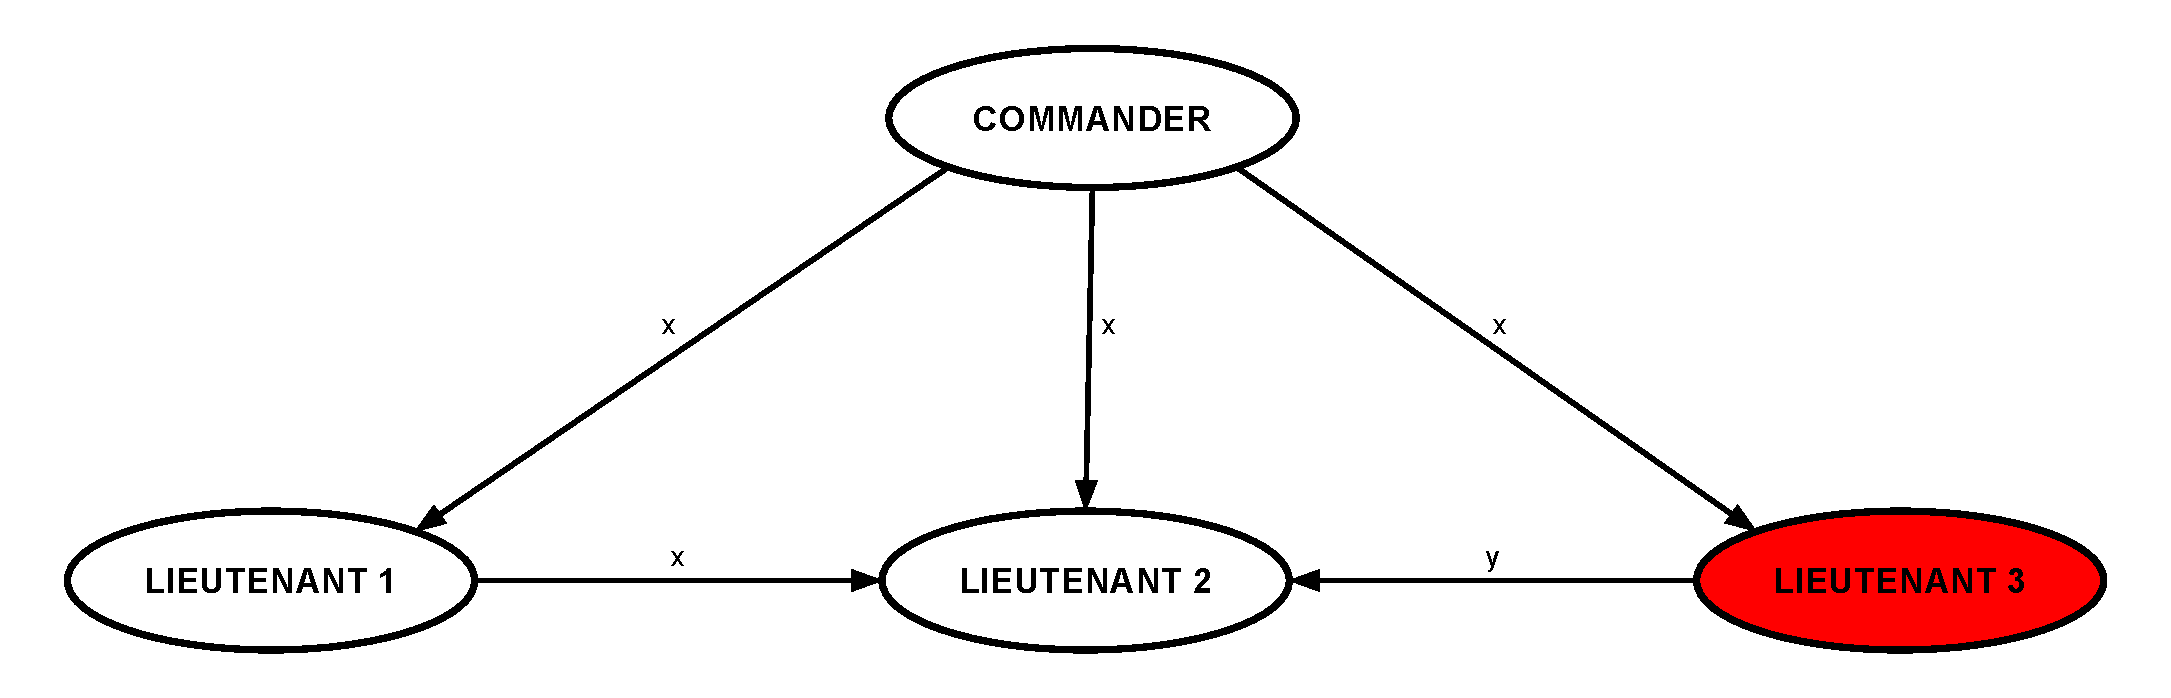
\includegraphics[scale=.32]{../figures/oral_messages_OM(1)_loyal_commander.pdf}
    \end{figure}
\end{frame}

\begin{frame}
    \frametitle{OM($m$) Commander is a Traitor}
    \begin{figure}
        \centering
        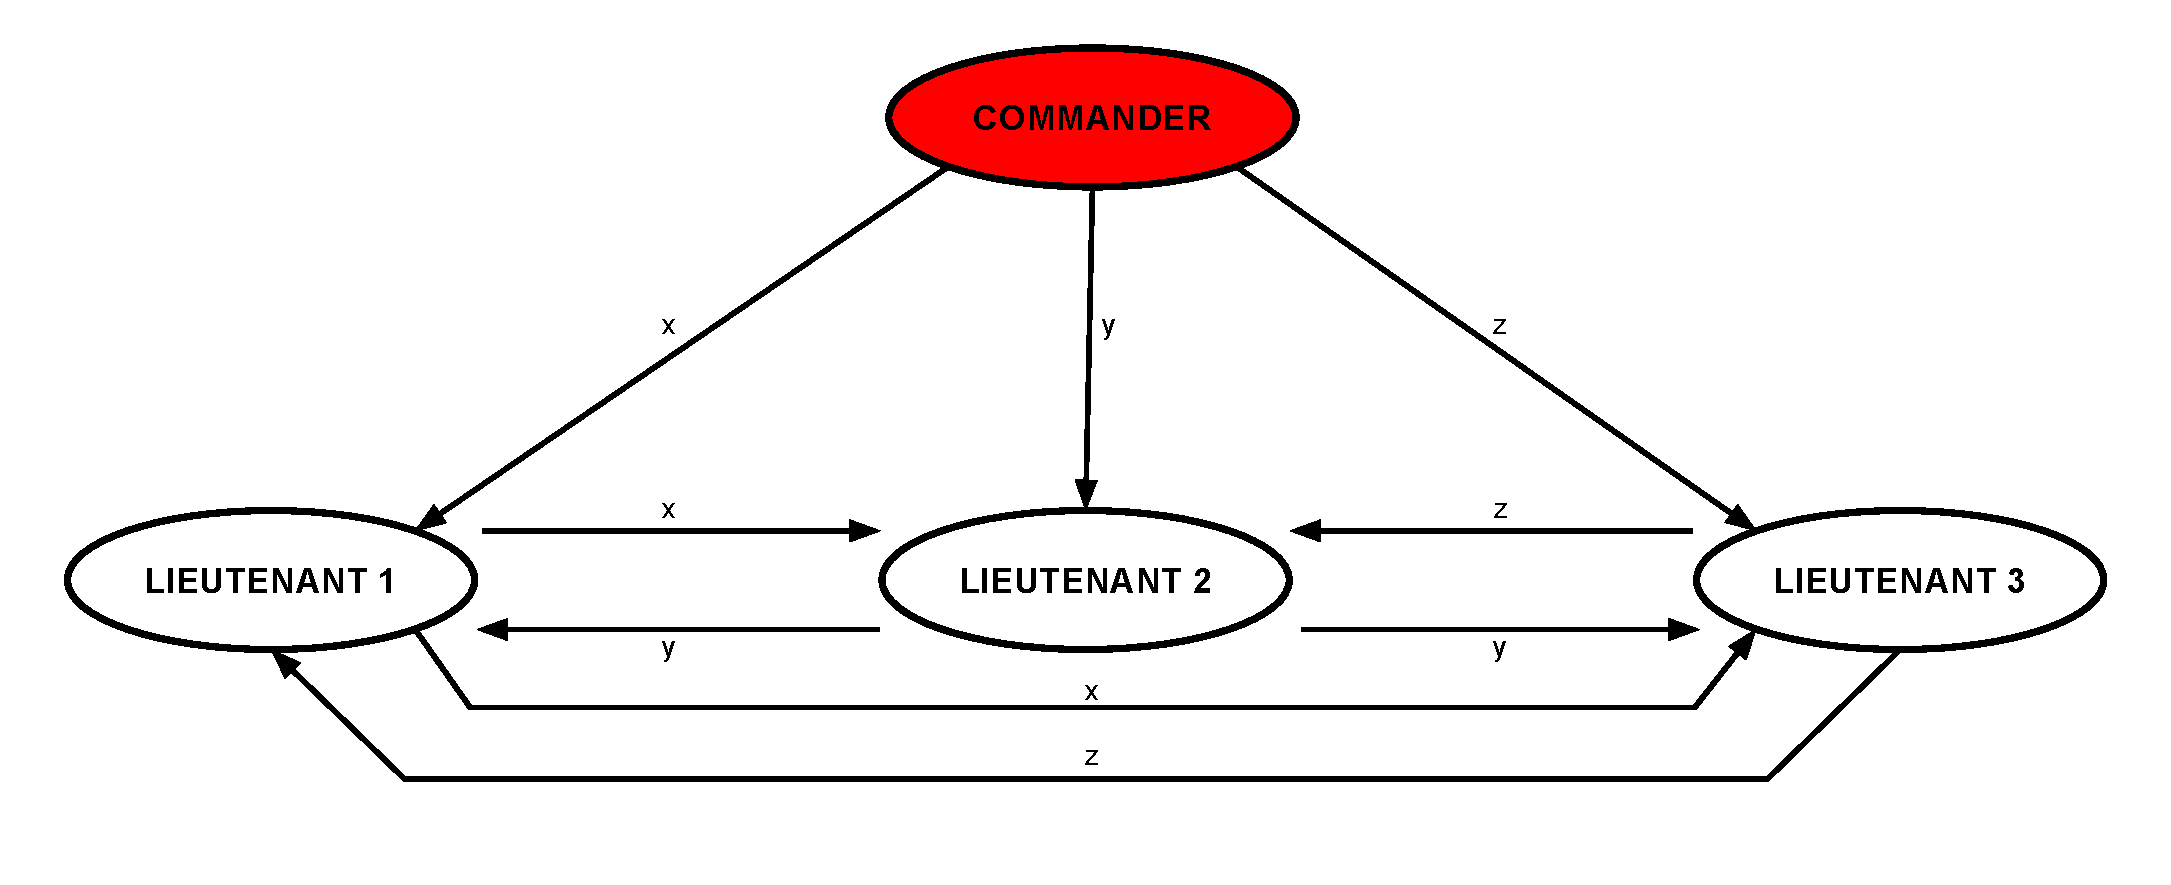
\includegraphics[scale=.32]{../figures/oral_messages_OM(1)_unloyal_commander.pdf}
    \end{figure}
\end{frame}


%%%%%%%%%%%%%%%%%%%%%%%%%%%%%%%%%%%%%%%%%%%%%%%%%%%%%%%%%%%%%%%%%%%%%%%%%%%%%%%%%%%%%%%%%%%%%%%%
%%  Signed Solution
%%%%%%%%%%%%%%%%%%%%%%%%%%%%%%%%%%%%%%%%%%%%%%%%%%%%%%%%%%%%%%%%%%%%%%%%%%%%%%%%%%%%%%%%%%%%%%%%

\section{Signed Messages}

\begin{frame}[t]
    \vfill
    \centering
    \begin{beamercolorbox}[sep=8pt,center,shadow=true,rounded=true]{title}
        \usebeamerfont{title}Signed Messages\par%
    \end{beamercolorbox}
\end{frame}

\begin{frame}
    \begin{enumerate}[label={A4.}]
        \item {
            \begin{enumerate}[label={(\alph*)}]
                \item<1-> {
                    A loyal general's signature cannot be forged, and any alterations of the contents of
                    their signed messages can be detected.
                }
                \item<2-> Anyone can verify the authenticity of a general's signature.
            \end{enumerate}
        }
    \end{enumerate}
\end{frame}

\begin{frame}
    We need some requirements for how the generals decide which order to follow:
    \begin{enumerate}[label={\arabic{enumi}.}]
        \item<2-> If the set $V$ consists of the single element $v$, then $choice(V) = v$.
        \item<3> $choice(\emptyset)=$ RETREAT, where $\emptyset$ is the empty set.
    \end{enumerate}
\end{frame}

\begin{frame}
    \begin{enumerate}[label={$\bullet$}]
        \item<1-> The value $x$ signed by General $i$ is denoted as $x:i$.
        \item<2> That means $x:i:j$ is the value $x$ signed by General $i$ and then General $j$.
    \end{enumerate}
\end{frame}

\begin{frame}
    \begin{block}{Algorithm SM($m$), $m>0$}
        Initially $V_i=\{\}$
        \begin{enumerate}[label=\arabic{enumi}.]
            \item<1-> The commander signs and sends their value to every lieutenant.
            \item<2-> For each $i$,
            \begin{enumerate}[label={\alph*.}]
                \item<3-> {
                    If Lieutenant $i$ receives a message from the commander of form $v:0$ and they have not received
                    any other order, then:
                    \begin{enumerate}[label=\roman*.]
                        \item<4-> they set $V_i=\{v\}$.
                        \item<5-> they send the message $v:0:i$ to every other lieutenant.
                    \end{enumerate}
                }
                \item<6-> {
                    If Lieutenant $i$ receives a message of the form $v:0:j_1:...:j_k$ and $v$ is not in $V_i$, 
                    then:
                    \begin{enumerate}[label=\roman*.]
                        \item<7-> they add $v$ to $V_i$.
                        \item<8-> {
                            if $k < m$, then they send the message $v:0:j_1:...:j_k:i$ to every other lieutenant,
                            except for $j_1,...,j_k$.
                        }
                    \end{enumerate}
                }
                \item<9-> {
                    For each $i$, when Lieutenant $i$ receives no more messages, they follow the result from 
                    $choice(V_i)$.
                }
            \end{enumerate}
            
        \end{enumerate}
    \end{block}
\end{frame}

\begin{frame}
    \frametitle{OM($m$) Commander is a Traitor}
    \begin{figure}
        \centering
        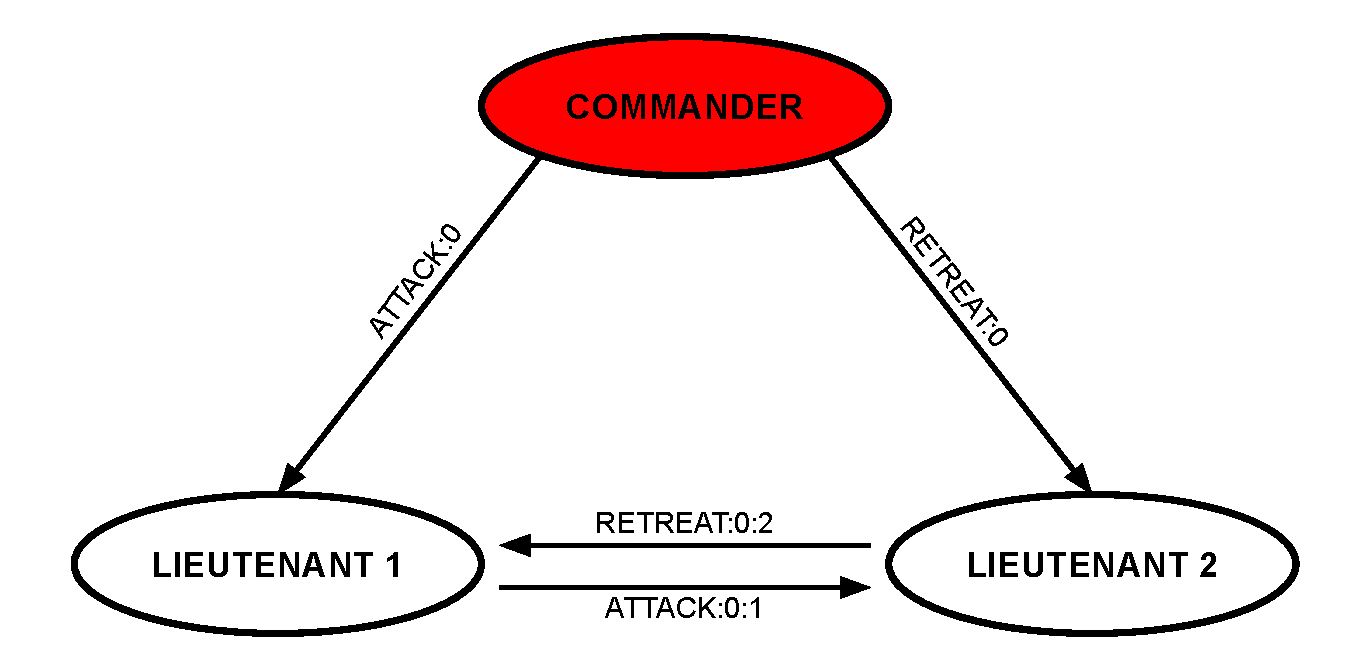
\includegraphics[scale=.5]{../figures/signed_messages_disloyal_commander.pdf}
    \end{figure}
\end{frame}


%%%%%%%%%%%%%%%%%%%%%%%%%%%%%%%%%%%%%%%%%%%%%%%%%%%%%%%%%%%%%%%%%%%%%%%%%%%%%%%%%%%%%%%%%%%%%%%%
%%  Conclusion
%%%%%%%%%%%%%%%%%%%%%%%%%%%%%%%%%%%%%%%%%%%%%%%%%%%%%%%%%%%%%%%%%%%%%%%%%%%%%%%%%%%%%%%%%%%%%%%%

\section{Conclusion}

\begin{frame}
    \frametitle{Applications}
    \begin{enumerate}[label={$\bullet$}]
        \item<1-> Computer components.
        \item<2-> Nodes on a network.
        \item<3> Blockchain
    \end{enumerate}
\end{frame}

%%%%%%%%%%%%%%%%%%%%%%%%%%%%%%%%%%%%%%%%%%%%%%%%%%%%%%%%%%%%%%%%%%%%%%%%%%%%%%%%%%%%%%%%%%%%%%%%
%%  References
%%%%%%%%%%%%%%%%%%%%%%%%%%%%%%%%%%%%%%%%%%%%%%%%%%%%%%%%%%%%%%%%%%%%%%%%%%%%%%%%%%%%%%%%%%%%%%%%

\frame{
    \frametitle{References}
    \begin{enumerate}{
        \scriptsize  
        \item[{[1]}] {
            L. Lamport, R. Shostak, and M. Pease, ``The Byzantine Generals Problem'', ACM Transactions on 
            Programming Languages and Systems, Vol. 4, No. 3, 1982, 382-401.
        }\item[{[2]}] {
            M. Pease, R. Shostak, and L. Lamport, ``Reaching agreement in the presence of faults.'', 
            J. ACM Transactions 27, 2, 1980, 228-234
        }
    }\end{enumerate}
}

\end{document}
